\documentclass{article}

% Language setting
% Replace `english' with e.g. `spanish' to change the document language
\usepackage[german]{babel}
\usepackage{xcolor}
\usepackage[dvipsnames]{xcolor}
% Set page size and margins
% Replace `letterpaper' with `a4paper' for UK/EU standard size
\usepackage[normalem]{ulem}
\usepackage[letterpaper,top=2cm,bottom=2cm,left=3cm,right=3cm,marginparwidth=1.75cm]{geometry}
\usepackage{amsthm}
\usepackage{amssymb}
% Useful packages
\usepackage{amsmath}
\usepackage{graphicx}
\usepackage[colorlinks=true, allcolors=blue]{hyperref}
\usepackage{float}

\usepackage{tikz}
\usetikzlibrary{positioning,arrows.meta}
\usepackage{biblatex}
\addbibresource{sample.bib}

\usepackage{tcolorbox}
\newtcolorbox{mybox}{colback=white,
colframe=Blue}
\title{Abgabe HUE 3}
\author{Liliana Sanfilippo}
\date{ {($\_\_\_$/20P)}}


\begin{document}
\maketitle 
\section*{Aufgabe 1 ($\_\_$/6P)}
Beschreiben Sie die Ergebnisse der folgenden Anfragen knapp und präzise. 
\begin{enumerate}
    \item $\pi_{PersonID, E-Mail}$(Person $\bowtie$ Review)
    \item $\pi_{Name, Jahr}$($\sigma_{PersonID=Autor \land Seiten\geq 100}$(Person $\times$ Buch))
    \item \(\pi_{\text{ISBN}}(\text{Buch}) - \pi_{\text{ISBN}}(\sigma_{\text{Sterne} \geq 3 \wedge \text{Sterne} \leq 7}(\text{Review}))\)
    \item \(G_{\text{count}}(\text{PersonID})(\pi_{\text{PersonID, ISBN}}(\text{Review}) \div \pi_{\text{ISBN}}(\text{Buch}))\)
    \item \(\pi_{\text{Name}}(\sigma_{\text{Jahr} = \text{Total}}(\text{Person} \bowtie \rho_{T(\text{PersonID, Total})}(\text{Autor} \ G_{\Sigma(\text{Seiten})}(\text{Buch}))))\)
    \item \[
\begin{aligned}
A &:= \sigma_{\text{Seiten} = \text{max}(\text{Seiten})}(\text{Buch} \times G_{\text{max}(\text{Seiten})}(\text{Buch})) \\
B &:= G_{\text{max}(\text{Seiten}), \text{min}(\text{Sterne})}(\text{Review} \bowtie A) \\
&\pi_{\text{Inhalt}}(\sigma_{\text{Seiten} = \text{max}(\text{Seiten}) \wedge \text{Sterne} = \text{min}(\text{Sterne})}(\text{Buch} \bowtie \text{Review} \times B))
\end{aligned}
\]
\end{enumerate}
\begin{mybox}

\begin{enumerate}
    \item Fragt eine Tabelle der Personen und deren E-Mail-Adressen ab, die einen Review geschrieben haben
    \item Fragt eine Tabelle der Autoren und deren Jahre ab, die Bücher mit mindestens 100 Seiten geschrieben haben 
    \item ISBNs aller Bücher die Reviews mit weniger als 3 oder mehr als 7 Sternen bekommen haben - also Bücher mit besonders guten oder schlechten Reviews
    \item  Die Anzahl der Personen die einen Review zu jedem Buch (aus der Buch-Tabelle) geschrieben haben 
    \item Fragt die Autoren ab (die auch in der Personen-Tabelle sind), bei denen Jahr der Anzahl der insgesamt geschriebenen Seiten entspricht
    \item Gibt den Inhalt der längsten Bücher mit den schlechtesten Bewertungen an  \\
    Anmerung: dabei geht es nicht um die x längsten oder x schlechtesten, sonder die Bücher die die maximal vorkommende Seitenzahl haben und die minimal vorkommende Anzahl von Sternen
\end{enumerate}
\end{mybox}
\section*{Aufgabe 2 ($\_\_$/6P)}
Formulieren Sie relationale Ausdrücke zu folgenden Anfragen:
\begin{enumerate}
    \item Bestimmten Sie die Autoren mit den längsten Büchern (ohne Aggregation G)
    \item Bestimmten Sie die Autoren mit den kürzesten Büchern (mit Aggregation G)
    \item Bestimmten Sie die Autoren mit den meisten Büchern
    \item Bestimmten Sie die Summe der Seiten aller Bücher ohne Reviews für alle Autoren
    \item Bestimmten Sie die durchschnittliche Anzahl an Seiten pro Buch für alle Autoren
    \item Bestimmen Sie die Inhalte der besten Reviews zu den kürzesten Büchern
\end{enumerate}
\begin{mybox}
\begin{enumerate}
    \item \( \pi_{Name}(\sigma_{Seiten=max(Seiten)}(Person \bowtie Buch)) \) 
    \item \(\pi_{Name}(\sigma_{Seiten=min(Seiten)}(G_{min(Seiten)}(Buch)))\)
    \item \(\pi_{Name}(\sigma_{Anzahl = max(Anzahl)}(Person \bowtie \rho_{Anzahl}(Autor\ G_{count}(Buch \bowtie Person))))\)
    \item Anmerkung: Ich interpretiere die Formulierung als man soll die Anzahl der Seiten der Bücher ohne Review für alle der Autoren zusammen berechnen \\
    \(G_{sum(Seiten)}(Buch - (Buch \bowtie Review))\)
    \item Anmerkung: Erneut, ich interpretiere da für alle Autoren zusammen genommen \\
    \( \pi_{avg(Seiten)}(Buch) \)
    \item 
  \[  \begin{aligned}
A &:= \sigma_{\text{Seiten} = \text{min}(\text{Seiten})}(\text{Buch} \times G_{\text{min}(\text{Seiten})}(\text{Buch})) \\
B &:= G_{\text{min}(\text{Seiten}), \text{max}(\text{Sterne})}(\text{Review} \bowtie A) \\
&\pi_{\text{Inhalt}}(\sigma_{\text{Seiten} = \text{min}(\text{Seiten}) \wedge \text{Sterne} = \text{max}(\text{Sterne})}(\text{Buch} \bowtie \text{Review} \times B))
\end{aligned}\]
\end{enumerate}
\end{mybox}
\section*{Aufgabe 3 ($\_\_$/6P)}
Überführen Sie das folgende E-R-Diagramm in das relationale Modell. Bestimmen Sie alle entstehenden Fremdschlüssel-Beziehungen und unterstreichen Sie alle Schlüsselattribute.
\begin{figure}[h]
    \centering
    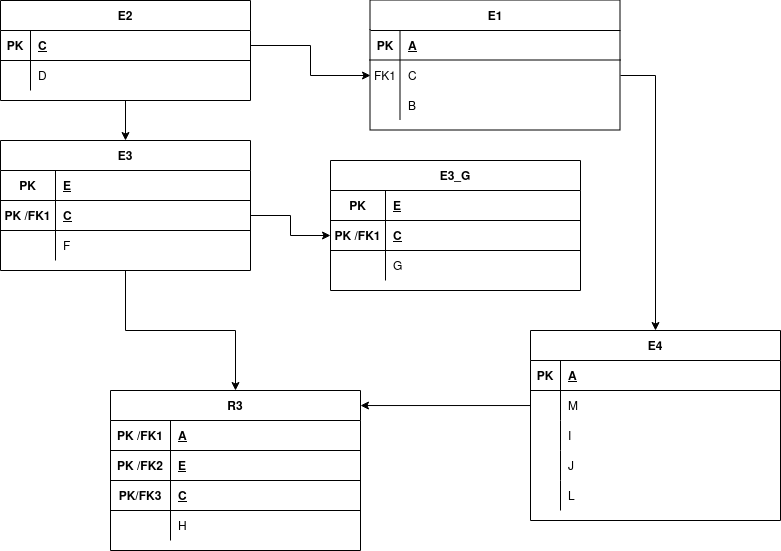
\includegraphics[width=\textwidth]{hue3.png}
\end{figure}
\section{Aufgabe 4 ($\_\_$/2P)}
ormulieren Sie passende SQL-Ausdrücke zu folgenden Anfragen.
\begin{enumerate}
    \item Bestimmen Sie alle Personen, welche genau zwei Reviews verfasst haben
    \item Bestimmen Sie die Summe der Sterne aller Reviews von Personen, die keine Autoren sind
\end{enumerate}
\begin{mybox}
\begin{enumerate}
    \item SELECT Person.PersonID FROM Person JOIN Review ON Person.PersonID = Review.PersonID GROUP BY Person.PersonID, Person.Name HAVING COUNT(Review.ReviewID) = 2
    \item SELECT SUM(Review.Sterne) AS SummederSterne FROM Review JOIN Person ON Review.PersonID = Person.PersonID WHERE Person.PersonID NOT IN (SELECT Autor.PersonID FROM Autor)

\end{enumerate}
\end{mybox}
\end{document}